\chapter{Cadyts}
\label{ch:cadyts}
\kaitodo[inline]{read chapter/section}
% ##################################################################################################################

\hfill \textbf{Authors:} Kai Nagel, Michael Zilske, Gunnar Fl\"otter\"od

\begin{center} 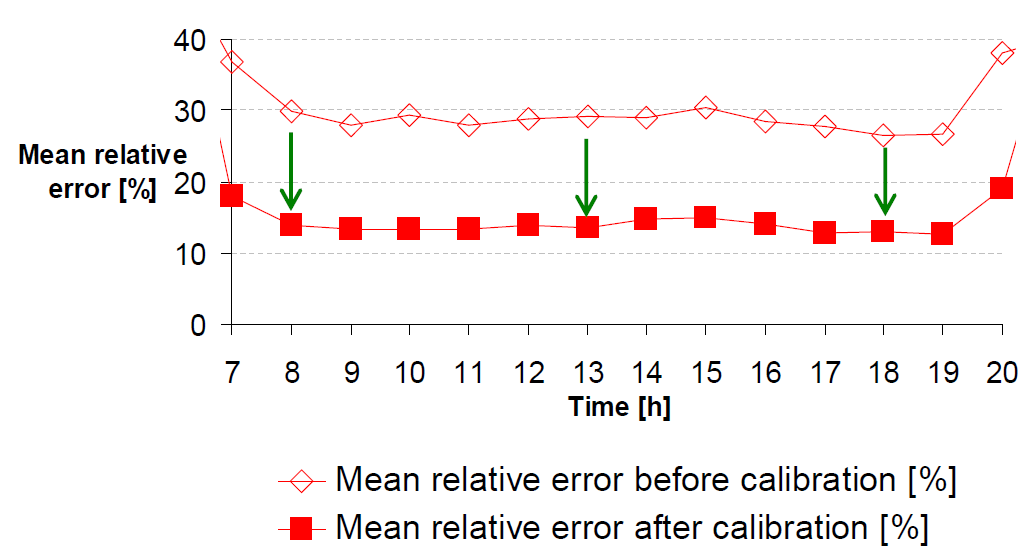
\includegraphics[width=0.5\textwidth, angle=0]{extending/figures/cadyts/cadyts} \end{center}

\editdone{This text has undergone the professional edit. Please no grammatical changes anymore! They are most-probably wrong.}

\createStandardInformation{cadytsIntegration}
{\lstinline{RunCadyts4CarExample} class}
{cadytsCar}
{\citet[][]{cadyts-manual, floetteroed-2010e, FloetteroedChenEtAl2011BehavioralCalibAndAnaNETS, Floetteroed2008PhD, Moyo2013PhD}}

% ##################################################################################################################

%\ah{adopted from \citet[][]{Floetteroed2009CadytsSTRC}. Please check, in particular copy rights of figure}
%\gunnar{Checked. -- Die Abbildung taucht in dem NETS paper gar nicht auf. Sollte so gesehen unproblematisch sein.}
%\ah{ok}

% ##################################################################################################################
\section{Introduction}

\gls{cadyts}\footnote{\url{http://people.kth.se/~gunnarfl/cadyts.html}}
--licensed under \gls{gplv3}--calibrates disaggregate travel demand models 
of \gls{dta} simulators from traffic counts and vehicle re-identification data. 
\gls{cadyts} is broadly compatible with \gls{dta} microsimulators,
into which it can be hooked through sparse interfaces.

As explained formally in Chapter~\ref{ch:abta} and~\ref{ch:montecarlo},
\gls{dta} \corr{targets}{aims at} consistency between a \corr{travel demand
dynamic}{dynamic travel demand} model\corr{--- matsim, represented by the
agents' plans---}{, defining the choice of activity-travel plans,} and a
\corr{network supply dynamic model}{dynamic network supply model}, capturing
spatiotemporal network flows and congestion evolution.

\gls{cadyts} adjusts \corr{all agents' plan choice probabilities}{the plan
choice probabilities of all agents}, resulting in
simulated network conditions \corr{}{that are} consistent with measured
real-world data\corr{,}{} while maintaining \corr{}{the} behavioral plausibility
of the underlying travel demand model.
Within MATSim, plan choice probabilities adjustment is realized 
by adjusting plan scores, as explained in the next section.

% ##################################################################################################################
\section{Adjusting Plans Utility}

When traffic counts are the empirical source, plan-specific score corrections 
are composed of link- and time-additive terms $\Delta S_a(k)$ for each link $a$
and each calibration time step $k$ (often one hour). 
When congestion is light and traffic counts are independently and normally distributed, 
these correction terms become 
%\cite[p.487]{FloetteroedChenEtAl2011BehavioralCalibAndAnaNETS}
%
\begin{equation}
\label{eq:cadyts:correction}
\Delta S_a(k) = \frac{y_a(k) - q_a(k)} {\sigma_a^2(k)}
\end{equation}
%
where $y_a(k)$ is \corr{}{the} real-world measurement on link $a$ in time step
$k$, $q_a(k)$ is its simulated counterpart and $\sigma^2_a(k)$ is (an estimate of) 
the real measurement variance  (assuming its expected value 
coincides with the prediction $q_a(k)$ of a perfectly calibrated simulator).

\corr{Score}{The score} correction of an agent's given activity-travel plan is
calculated as the sum of all $\Delta S_a(k)$, \corr{when}{given that} following
that plan implies entering link $a$ within time step $k$.
% \citep{FloetteroedChenEtAl2011BehavioralCalibAndAnaNETS}.
With this, the \textit{a posteriori} choice probability of agent $n$'s plan
$i$\corr{,}{} given the count data ${\bf y} = \{y_a(k)\}$\corr{,}{}
becomes\corr{:}{}
\begin{equation}
P_n(i\mid{\bf y}) \sim 
\exp\left(S_n(i)+ \sum_{ak\in_{}i} \Delta S_a(k) \right)
\,\,=\,\,
\exp\left(S_n(i)+ \sum_{ak\in_{}i} \frac{y_a(k) - q_a(k)} {\sigma_a^2(k)} \right)
\label{eq:cadyts:selection}
\end{equation}
where $S_n(i)$ is the \textit{a priori} score of plan $i$ of agent $n$, as 
calculated\corr{--}{ }for example\corr{--}{ }with Equation~(\ref{eq:matsimUTF}) and $ak\in
i$ reads:
``following plan $i$ implies entering link $a$ in time step $k$''.

Intuitively, if the \corr{simulation}{simulated} value $q_a(k)$ is smaller than
the real measurement $y_a(k)$, then a score increase, and thus a \corr{choice
increase probability}{choice probability increase}, results.
\corr{}{The variance} $\sigma^2_a(k)$ denotes \corr{}{the} level of trust in
that specific measurement --\ a large \corr{variance}{} $\sigma^2_a(k)$ implies
\corr{}{a} low trust level, taking effect through a large denominator in the
corresponding score correction addend.

\citet[][]{floetteroed-2010e} is the key methodological reference on \gls{cadyts}.
\corr{Its calibration approach is derived from a Bayesian argument,
providing}{It derives the calibration approach from a Bayesian argument and
provides} more technical information, such as a more general \corr{functional
utility form correction}{correction of the utility function than} in
Equation~(\ref{eq:cadyts:correction})\corr{,}{} that also applies when congestion
is present.
A  lighter presentation is 
\citet[][]{FloetteroedChenEtAl2011BehavioralCalibAndAnaNETS}, where the 
formulas above are discussed in somewhat greater detail.

% ##################################################################################################################
\section{Hooking Cadyts Into MATSim}
Hooking \gls{cadyts} into \gls{matsim} is based on the following operations:
\begin{enumerate}\styleEnumerate
\item Initialization: When the calibration is started, it requires all available 
traffic counts and some further parameters. 
For this, the \gls{cadyts} function \lstinline|void addMeasurement(...)| is called once for every 
measurement\corr{,}{} before the simulation starts. It registers a certain
measurement type, which has been observed on a specific link.
\item Iterations: The calibration is run jointly with the simulation until (calibrated) 
stationary conditions are reached.
	\begin{enumerate}[label=\emph{\alph*})]
	\item Demand simulation: The calibration needs an access point in the simulation 
	to affect the plan choice. There are various ways to realize this, depending on the  
	simulator.	
	%\gunnar{Trifft Folgendes f\"ur MATSim zu? Ich habe diesen Funktionsaufruf aus der
	%CadytsScoring-Klasse herausgefischt, bin mir aber nicht sicher, wie das auf der MATSim-Seite
	%zusammenspielt.}
	%\ah{m.E. geschieht genau das in \lstinline|org.matsim.contrib.cadyts.general.CadytsPlanChanger.selectPlan(...)|}\kai{Ja.  Noch einfacher in CadytsScoring.}
	Before a \gls{matsim} agent chooses a plan, \corr{he or she}{it} asks the
	calibration through the \gls{cadyts} function
	\lstinline|double calcLinearPlanEffect(Plan plan)| for all of its plans' score offsets.
    The agent then chooses a plan based on accordingly modified scores.
	\item Supply simulation: The calibration must observe simulated network conditions 
  to evaluate their deviation from real traffic counts.
	For this, the \gls{cadyts} function \lstinline|void afterNetworkLoading(SimResults simResults)| 
	is called once after each network loading. It passes a container object to the calibration
	\corr{, providing}{that provides} information about \corr{}{the} most recent
	network loading results, particularly on simulated flows at measurement locations.
	\end{enumerate}
\end{enumerate}

% ##################################################################################################################
\section{Applications}
\gls{cadyts} has been successfully applied in studies like % FloetteroedEtAl2009IatbrCalibration, 
\citet[][]{ZiemkeNagelBhatIntegratingCemdapMatsimTransferability,ZilskeNagelPhoneTracesAndCadyts, FloetteroedChenEtAl2011BehavioralCalibAndAnaNETS}. 
Zürich scenario results illustrate its efficiency, as shown in \citet[][Slide~8]{FloetteroedEtAl_unpub_MATSimUserMeeting_2011}, 
reproduced in Figure~\ref{fig:cadyts}.

\createfigure%
{Zürich case study results: mean relative error in link volumes}%
{Zürich case study results: mean relative error in link volumes}%
{\label{fig:cadyts}}%
{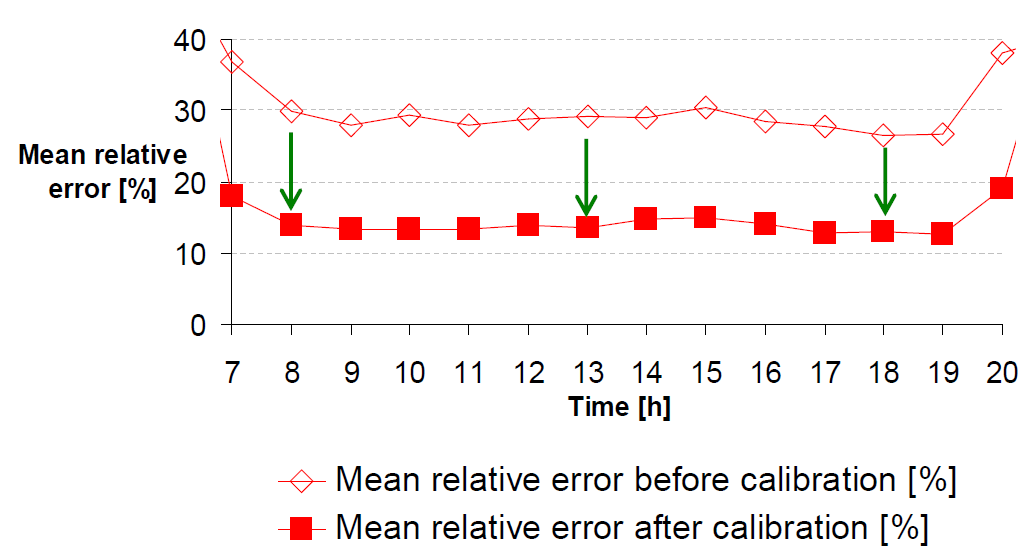
\includegraphics[width=0.8\textwidth, angle=0]{extending/figures/cadyts/cadyts}}%
{\citet[][Slide~8]{FloetteroedEtAl_unpub_MATSimUserMeeting_2011}}

% ##################################################################################################################
% Local Variables:
% mode: latex
% mode: reftex
% mode: visual-line
% TeX-master: "../../main"
% comment-padding: 1
% fill-column: 9999
% End: 
